






% =========----------	[ Space left here for distraction free mode] ----------==========%









\subsection{Analysis 4: Is there a difference in perception of timbre with difference viewing positions?}
	
	To assess whether viewing angle affected peoples perception of timbre, microphones that were used across both tests (spot mics on their own and microphones from position C) were directly compared for each of the timbral attributes. Figure~\ref{image:ta_sharedmics} shows a the percentage of participants that selected each timbral attribute for each microphone the figures for which is shown in table~\ref{ana4:perDiff}.

	The sway column is calculated by taking the average non-absolute average of the percentage differences for each timbral attribute. This indicates whether the timbral attribute was more frequently selected when viewing from position A (positive number) or positions B (negative number).

	It can be seen that the TA 'Realistic' experienced the greatest variation between viewing positions with an average of 20\% more participants selecting that viewing angle A 

	The TA's 'Rich' and 'Realistic' both experienced an average percentage difference 

	% FINISH THIS SECTION

	% \begin{math}
	% 	Sway = 	\frac{\sum_{n=1}^{N} {p}}{N}\\
	% \end{math}

	The 'Sway' column is calculated by summing the individual percentage difference for each timbral attribute resulting in a scalar representing which viewing position had a greater number of participants choosing each of the timbral attributes, where a positive number represents A and a negative number represents B.



	\begin{center}
	\begin{table}
		\begin{tabular}{r >{\centering\arraybackslash}p{30mm} c}
			Attribute & Absolute Average Percentage Difference & Sway \\
			Full & 7.89 & -1.32 \\
			Bright & 10.53 & -5.26 \\
			Flat & 9.21 & -6.58 \\
			Rich & 20.39 & 12.5 \\
			Realistic & 19.08 & 19.08 \\
			Loud & 6.58 & 6.58 
		\end{tabular}
		\caption{Percentage difference}
		\label{ana4:perDiff}
	\end{table}
	\end{center}


	
	\begin{figure}
		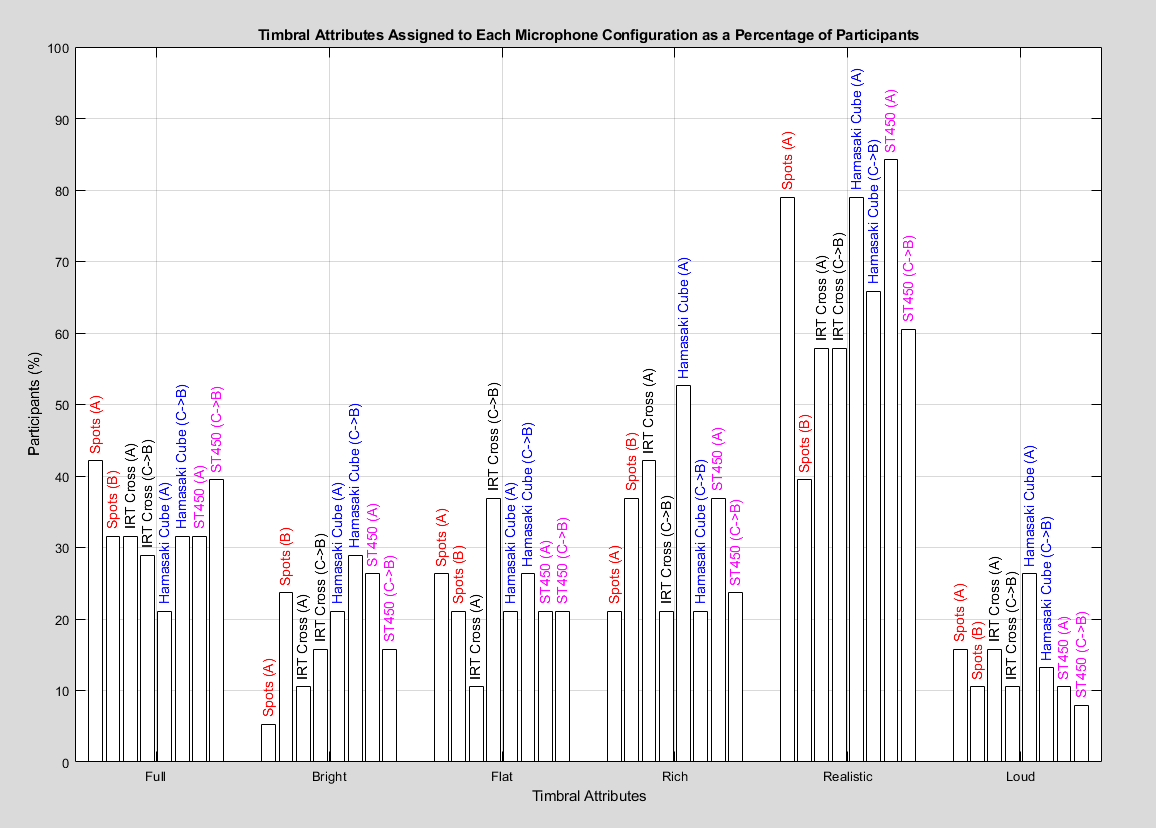
\includegraphics[width=0.5\textwidth]{images/plots/bar_sharedMics.PNG}
		\caption{Bar chart showing the timbral attributes chosen for each microphone array shared between viewing position A and B as a percentage of participants}
		\label{image:ta_sharedmics} 
	\end{figure}		

